\documentclass{article}
\usepackage{graphicx}
\usepackage[margin=1in]{geometry}
\usepackage[usenames, dvipsnames]{color}


\begin{document}

\title{Supplementary material for ``Visualization methods for RNA-sequencing data analysis"}
  \author{Lindsay Rutter}
  
  \maketitle
  
  This file contains supplementary analyses that the reader might find useful, and that extend upon several of the main concepts discussed in the paper. We include additional examples of how parallel coordinate plots, scatterplots matrices, and litre plots can be used to assess normalization and DEG calls. Below we provide a brief description of the first seven figures in this supplementary file:
  
  \begin{itemize}
  
  \item Figure~\ref{sbIRClusters} shows parallel coordinate plots of hierarchical clusters in a similar manner as Figure 2 in the main paper. The data comes from the iron-metabolism soybean study, and has been filtered and standardized. However, unlike Figure 2 in the main paper only showing significant genes, Figure~\ref{sbIRClusters} in this supplementary file shows all genes.
  
  \item Figure~\ref{mdsSwitch} shows that some of the most popular RNA-seq visualization tools cannot always detect common errors, such as sample switching. Side-by-side boxplots and MDS plots are shown for the soybean cotyledon dataset after deliberately switching samples between treatment groups. For the most part, they are unable to detect the error. In contrast, the less-popular method of scatterplot matrices can quickly detect the possibility of the error (see Figure 5 from the main paper).
  
  \item Figure~\ref{soybeanDEG} shows that the number of DEGs drastically changes across three time points when comparing iron sufficient versus iron deficient conditions in soybean leaves (Lauter \textit{et al}., 2016). As a result, the authors of this study postulate that the streak of genes observed in the scatterplot matrix containing the subset of data at the 120 minute time point (Figure 6 in the main paper) may be due to the timing differences between replicate handling.
  
  \item Figures~\ref{sbIRClusterSigSM1} through~\ref{sbIRClusterSigSM4} show scatterplot matrices of the significant genes in the iron-metabolism soybean dataset for each of the four clusters that resulted from hierarchical clustering analysis. They provide an additional and complementary perspective on these DEG calls from what we saw with the parallel coordinate plots in Figure~\ref{sbIRClusters}. 
  
  \item Figure~\ref{litreCluster1} shows example litre plots for two significant genes from Cluster 1. The reader may wish to view it alongside Figure 8 from the main paper, which contains example litre plots for significant genes from Clusters 2, 3, and 4.
  
  \end{itemize}
  
  The last twenty figures in the supplementary file are all related to the application of normalization techniques to the liver and kidney technical replicate data that were introduced in Section 5 (Closing case study) of the main paper. These figures also introduce examples that demonstrate the effect of standardizing data before viewing them. A brief description of these twenty figures starts on Page 9.
  
  %%%%%%%%%%%%%%%%%%%%%%%%%%%%%
  %%%%%%%%%%%%%%%%%%%%%%%%%%%%%
  %%%%%%% Begin Figures %%%%%%% 
  
  \clearpage
  \null
  \begin{figure}[t!]
  \centerline{\includegraphics[width=\columnwidth]{../MakeFigures/sbIRClusters.jpg}}
  \caption{Example application of parallel coordinate plots using the iron-metabolism soybean dataset. We filtered genes with low means and/or variance, performed a hierarchical clustering analysis with a cluster size of four, and visualized the results using parallel coordinate lines. Most non-filtered genes were in Clusters 1 and 2, which both showed overexpression in one treatment and underexpression in the other treatment. The genes in Cluster 4 mostly showed messy patterns with low signal to noise ratios. Interestingly, Cluster 3 looked similar to Cluster 2 (large values for group N and small values for group P), except for unexpectedly large values for the third replicate of group P. The side-by-side boxplots represent \textit{all} gene counts in the dataset.
  \label{sbIRClusters}}
  \end{figure}
  
  \clearpage
  \null
  \begin{figure}[!t]
  \centerline{\includegraphics[width=0.7\columnwidth]{SupplementaryFigure2Dots.png}}
  \caption{Boxplots and MDS plots are popular plotting tools for RNA-seq analysis. This figure shows these traditional visualization methods applied to the soybean cotyledon data before sample switching (left half) and after sample switching (right half). We cannot suspect from the right boxplot that samples S1.3 and S2.1 have been swapped (subplots A). This is because all six samples have similar five number summaries. For the MDS plots, we do see a cleaner separation of the two treatment groups across the first dimension in the left plot than in the right plot (subplots B). However, taking into account the second dimension, both MDS plots contain three clusters, with sample S1.1 appearing in its own cluster. Without seeing one distinct cluster for each of the two treatment groups, it is difficult to suspect that samples S1.3 and S2.1 have been swapped in the right MDS plot (subplots B). We can only derive clear suspicion that the samples may have been switched by using less-popular plots that provide gene-level resolution like with the scatterplot matrix from Figure 6 in the main paper.
  \label{mdsSwitch}}
  \end{figure}
  
  \clearpage
  \null
  \begin{figure}[!t]
  \centerline{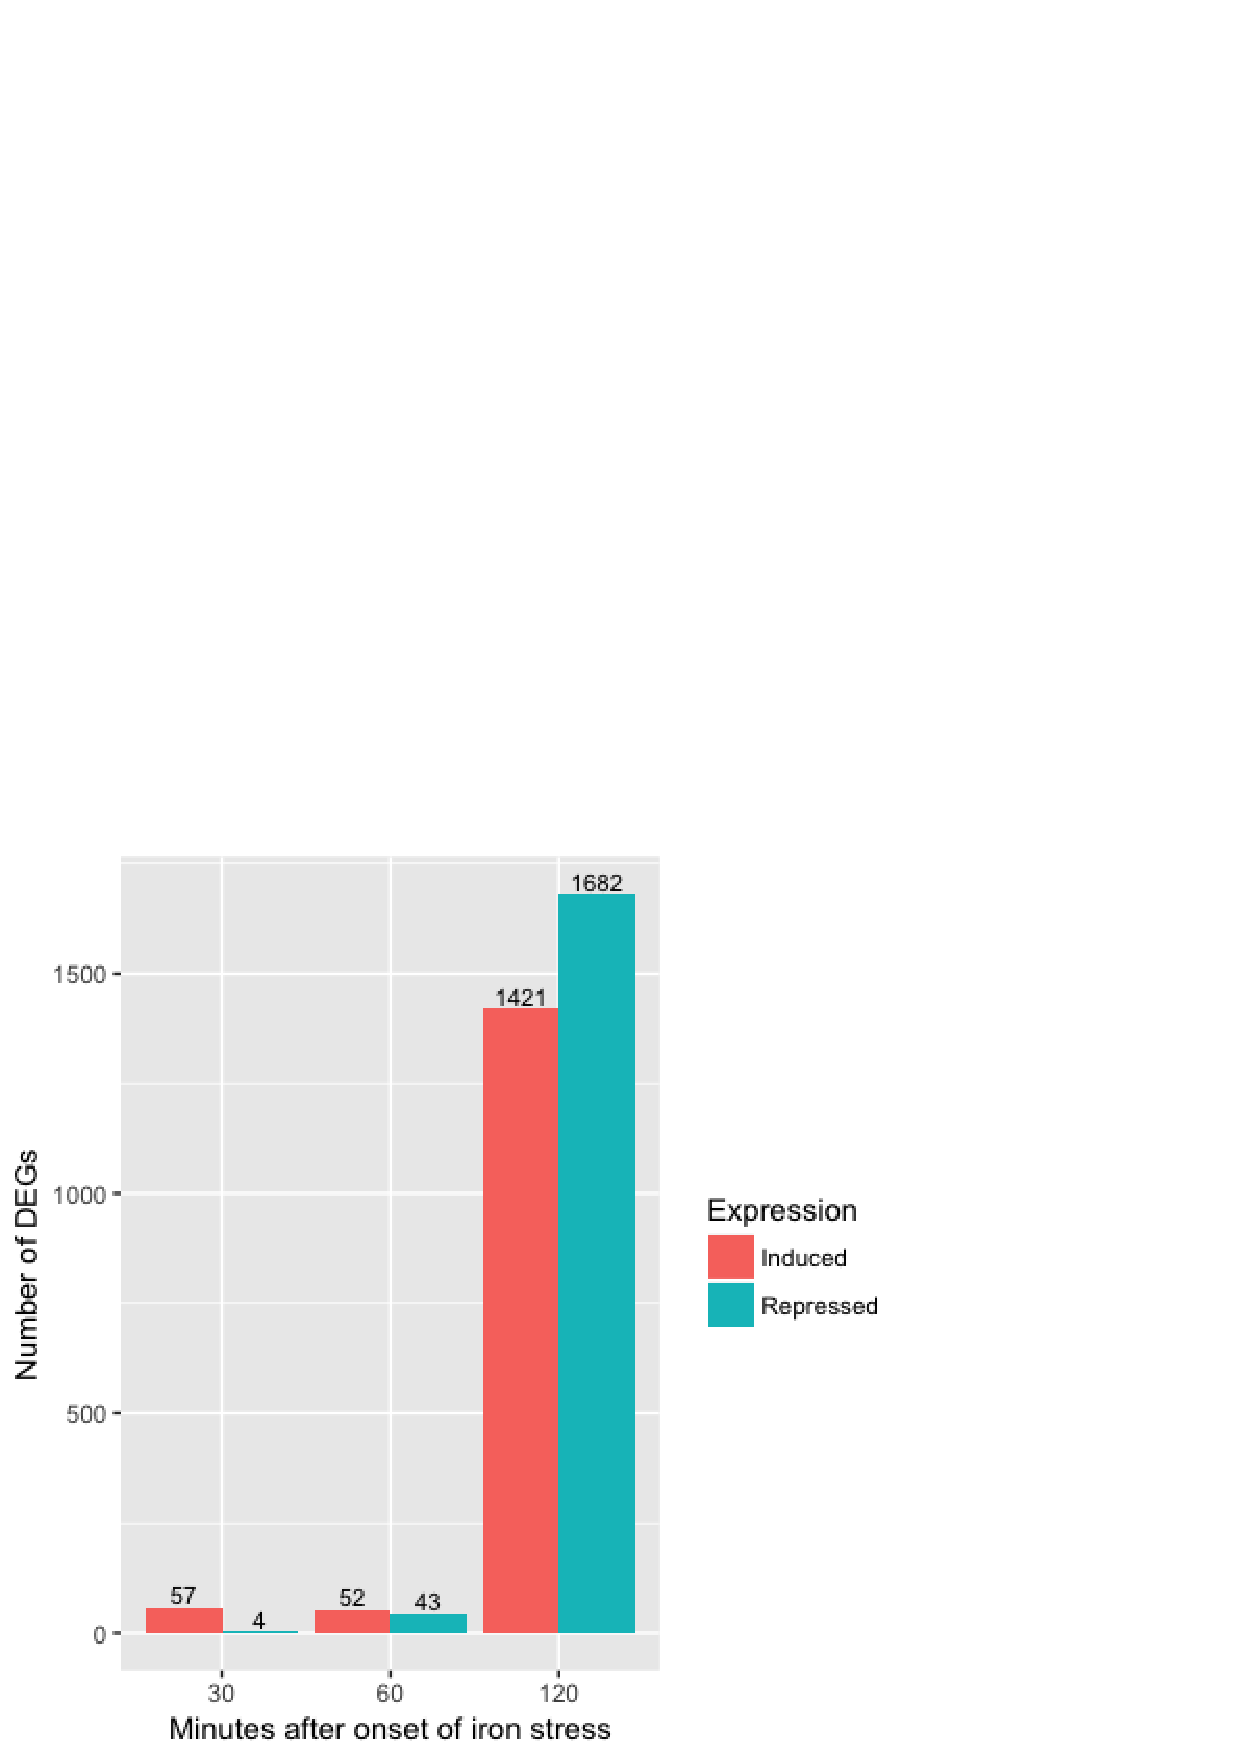
\includegraphics[width=0.7\columnwidth]{../MakeFigures/soybeanDEG.png}}
  \caption{The authors of the soybean iron metabolism study (Lauter \textit{et al}., 2016) determined the DEGs across three times points (30 minutes, 60 minutes, and 120 minutes) in the leaves after onset of iron sufficient and deficient hydroponic conditions. They used the same researcher to collect the samples in succession. One major finding from their study was a vaste change in gene expression responses between these three time points. As a result, the streak observed in the scatterplot matrix containing the subset of data at the 120 minute time point (Figure 6 in the main paper) may be due to the timing differences between replicate handling.
  \label{soybeanDEG}}
  \end{figure}
  
  \clearpage
  \null
  \begin{figure}[t!]
  \centerline{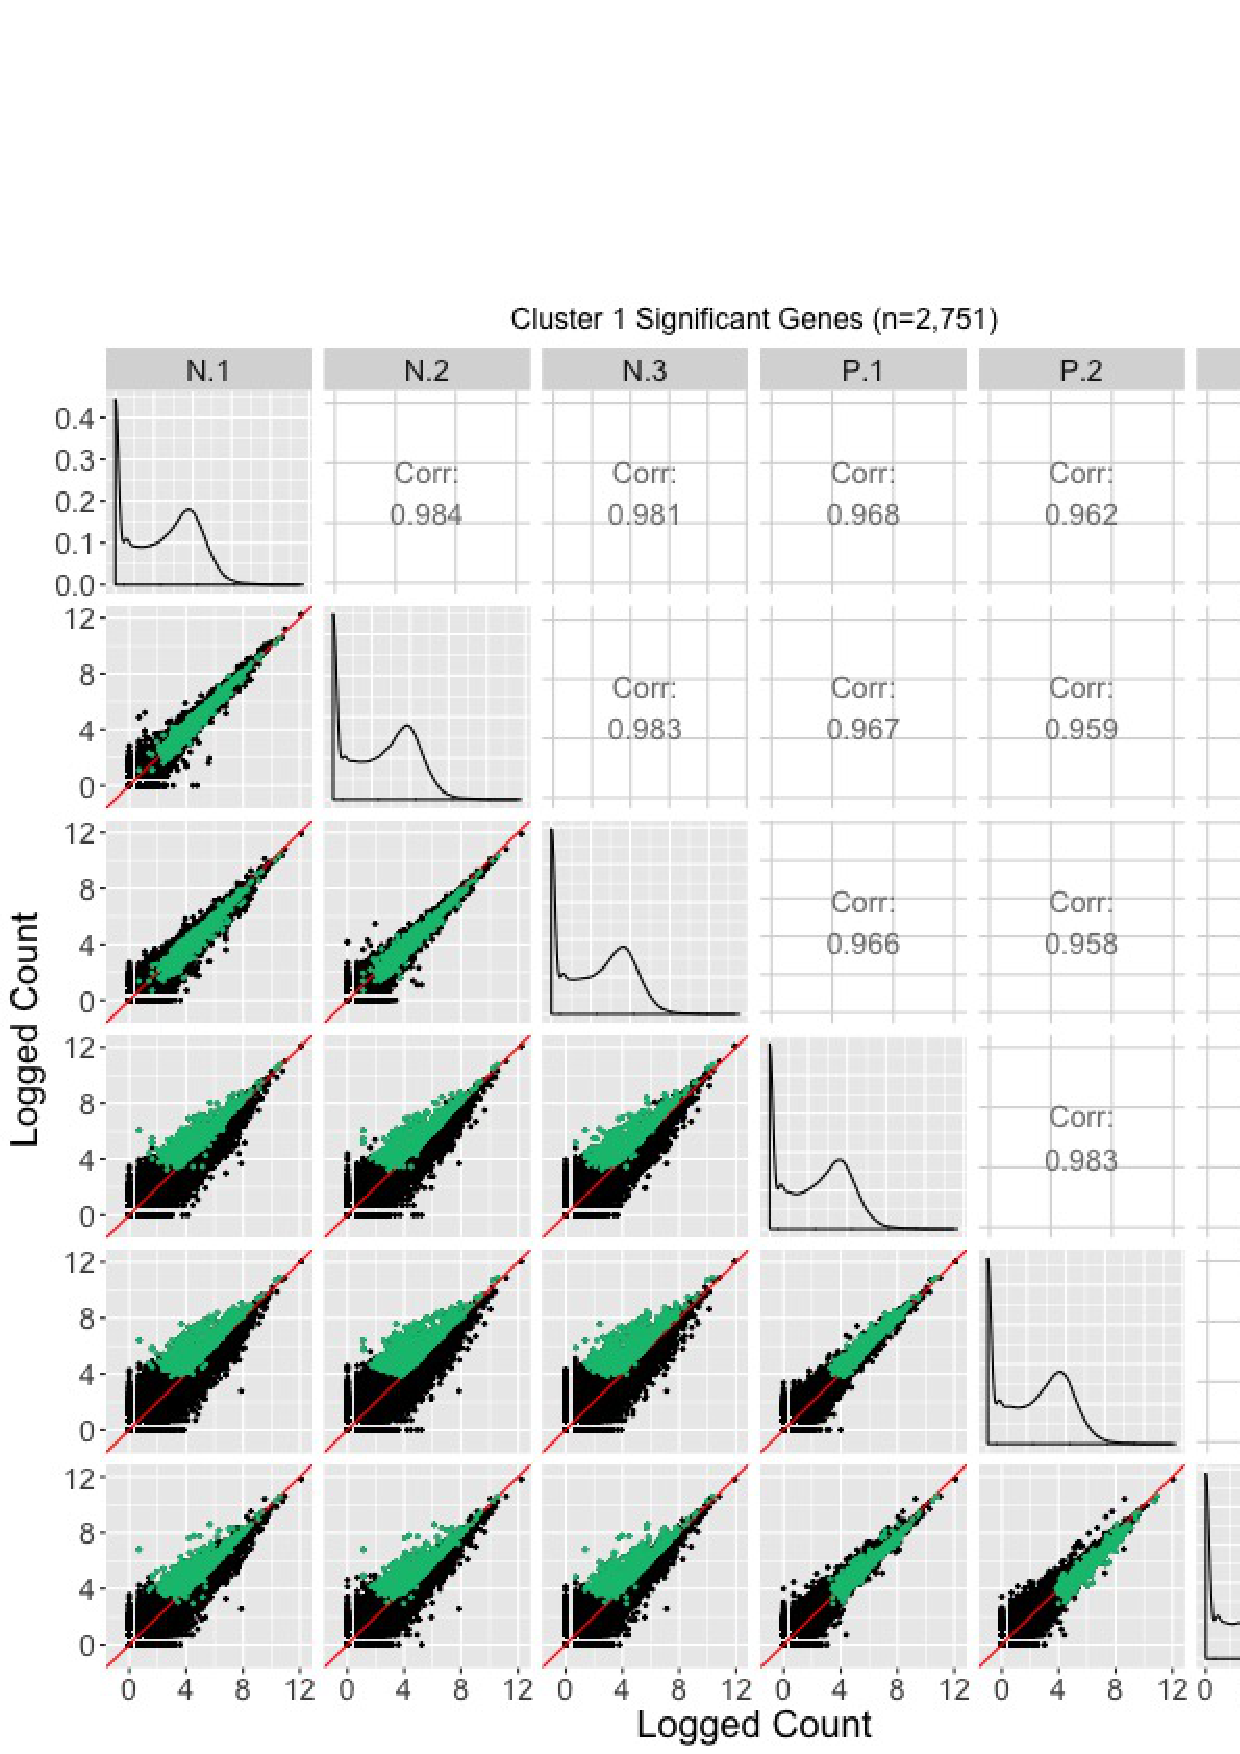
\includegraphics[width=\columnwidth]{../MakeFigures/sbIRClusterSigSM1.jpg}}
  \caption{Example of using a scatterplot matrix to assess DEG calls from a model in the iron-metabolism soybean dataset. There were 2,751 significant genes in Cluster 1 after performing a hierarchical clustering analysis with a cluster size of four (Figure 2 in the main paper). These significant genes are overlaid in green on the scatterplot matrix. They follow the expected patterns of differential expression with most green points falling along the \textit{x=y} line in the scatterplots between replicates, but deviating from the \textit{x=y} line in the scatterplots between treatments. The deviation consistently demonstrates higher expression in the P group than in the N group. Hence, these green points seem to represent genes that were significantly overexpressed in the P group, which draws the same conclusion with what we derived using the parallel coordinate plots in Figure 2 of the main paper. One difficulty with plotting such a large number of DEGs onto the scatterplot matrix is that overplotting can obscure our inability to determine how many DEGs are in a given location. This is why we might also view these genes individually in litre plots (Supplementary Figure 7).
  \label{sbIRClusterSigSM1}}
  \end{figure}
  
  %\null
  \begin{figure}[h!]
  \centerline{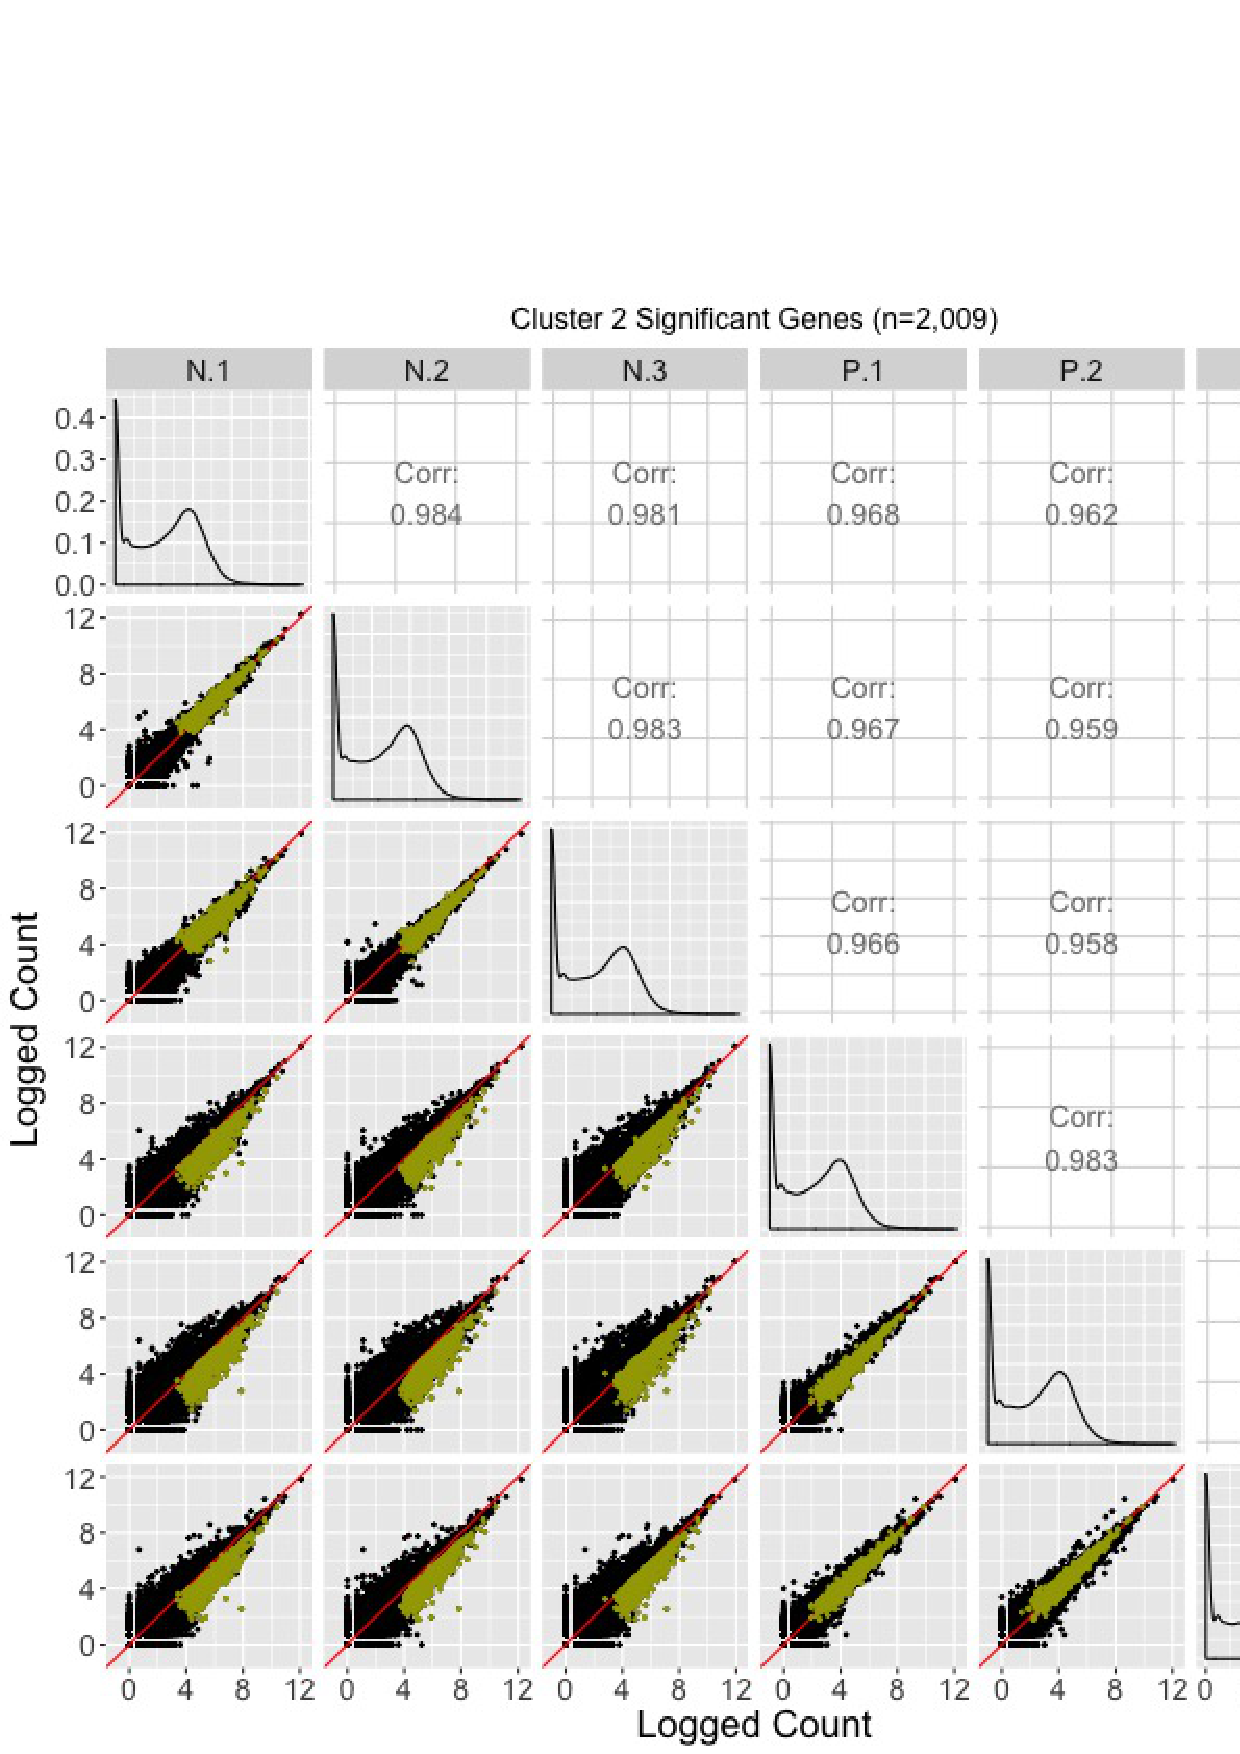
\includegraphics[width=\columnwidth]{../MakeFigures/sbIRClusterSigSM2.jpg}}
  \caption{Example of using a scatterplot matrix to assess DEG calls from a model in the iron-metabolism soybean dataset. There were 2,009 significant genes in Cluster 2 after performing a hierarchical clustering analysis with a cluster size of four (Figure 2 in the main paper). These significant genes are overlaid in dark yellow on the scatterplot matrix. They follow the expected patterns of differential expression with most dark yellow points falling along the \textit{x=y} line in the scatterplots between replicates, but deviating from the \textit{x=y} line in the scatterplots between treatments. The deviation consistently demonstrates higher expression in the N group than in the P group. Hence, these dark yellow points seem to represent genes that were significantly overexpressed in the N group, which draws the same conclusion with what we derived using the parallel coordinate plots in Figure 2 of the paper. One difficulty with plotting such a large number of DEGs onto the scatterplot matrix is that overplotting can obscure our inability to determine how many DEGs are in a given location. This is why we might also view these genes individually in litre plots (Figure 8 A and B in the main paper).
  \label{sbIRClusterSigSM2}}
  \end{figure}
  
  \null
  \begin{figure}[t!]
  \centerline{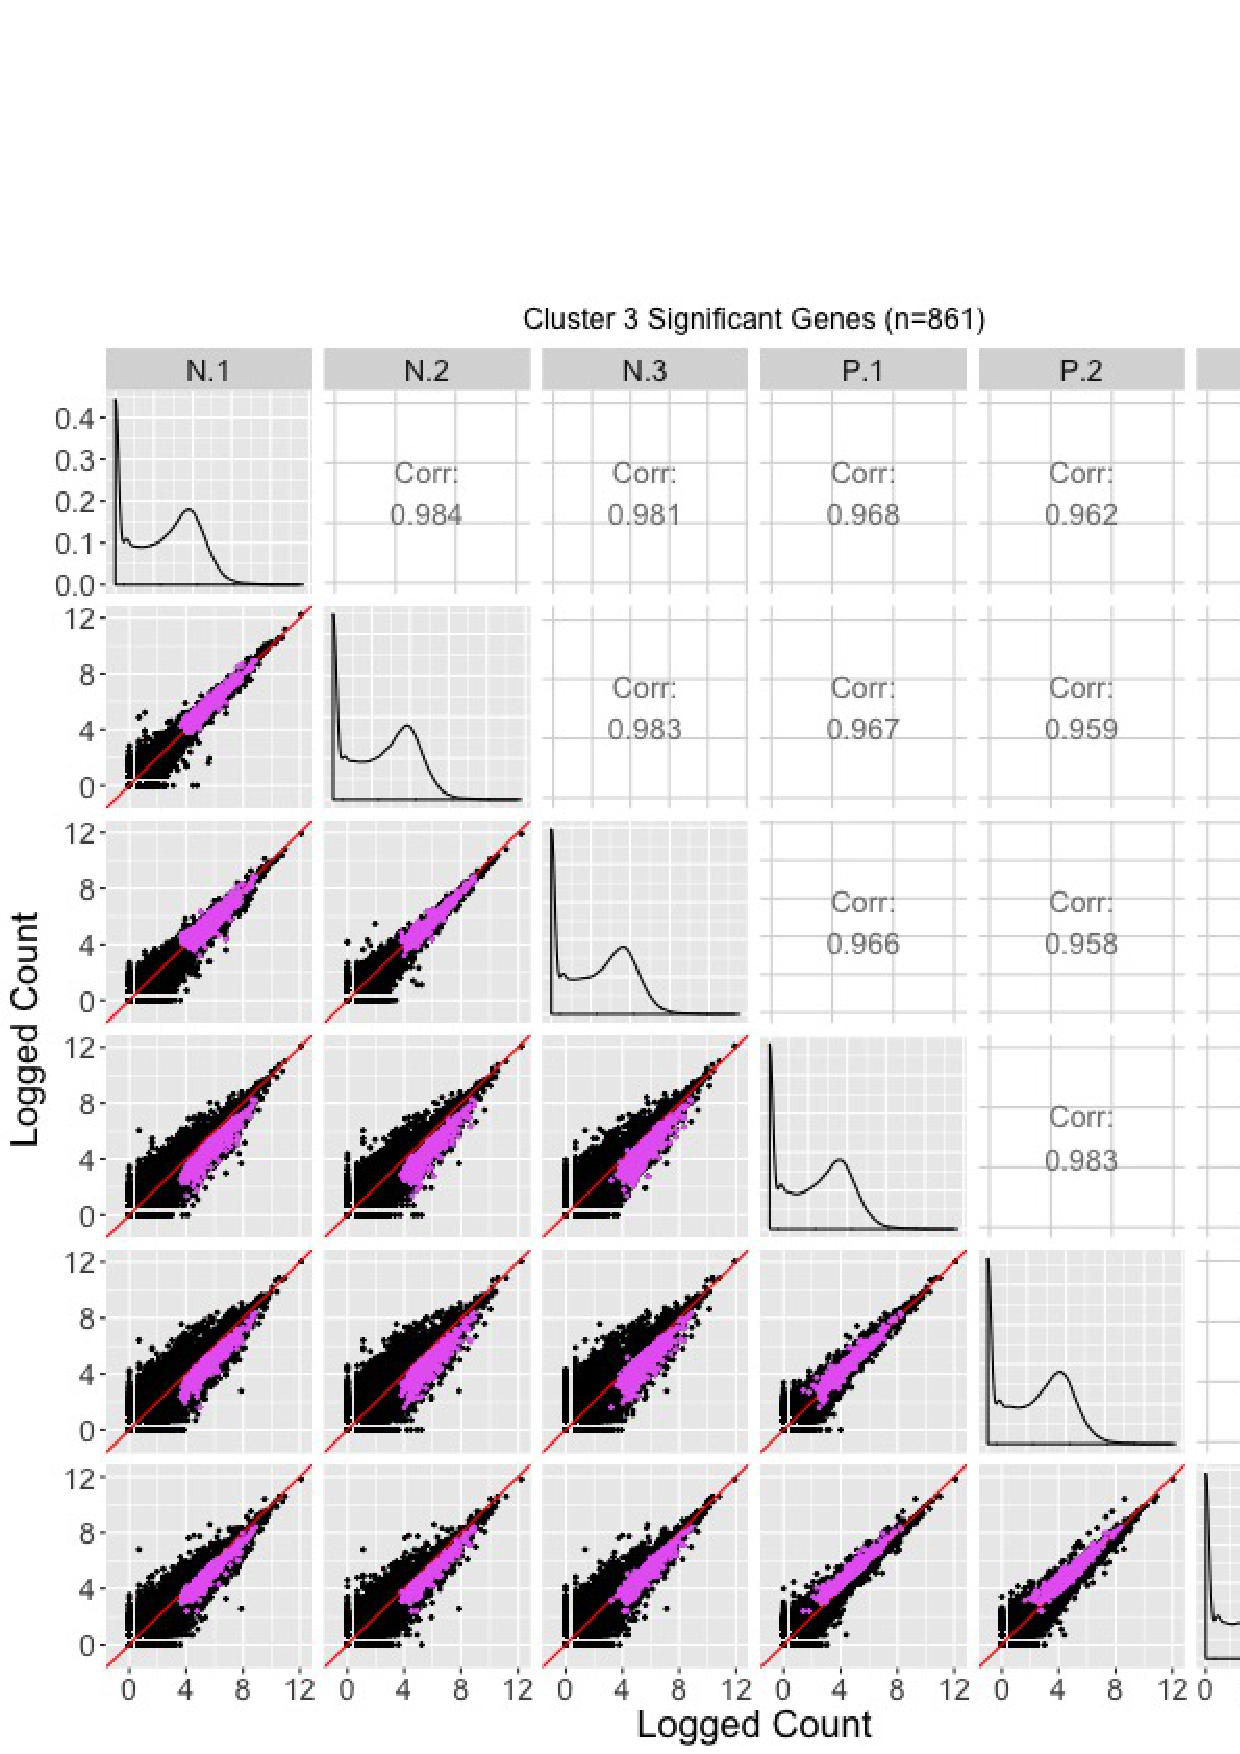
\includegraphics[width=\columnwidth]{../MakeFigures/sbIRClusterSigSM3.jpg}}
  \caption{Example of using a scatterplot matrix to assess DEG calls from a model in the iron-metabolism soybean dataset. There were 861 significant genes in Cluster 3 after performing a hierarchical clustering analysis with a cluster size of four (Figure 2 in the main paper). These significant genes are overlaid in pink on the scatterplot matrix. For the most part, they follow the expected patterns of differential expression with pink points falling along the \textit{x=y} line in the scatterplots between replicates, but deviating from the \textit{x=y} line in the scatterplots between treatments. The deviation consistently demonstrates higher expression in the N group than in the P group. However, the scatterplot between replicates P.1 and P.3 shows slightly higher expression in P.3, and the scatterplot between replicates P.2 and P.3 also shows slightly higher expression in P.3. Hence, these pink points seem to represent genes that were significantly overexpressed in the N group, but with slight inconstencies in the replicates in the P group. The parallel coordinate plots in Figure 2 of the paper showed this same conclusion and perhaps more clearly. One difficulty with plotting such a large number of DEGs onto the scatterplot matrix is that overplotting can obscure our inability to determine how many DEGs are in a given location. This is why we might also view these genes individually in litre plots (Figure 8 C and D in the main paper).
  \label{sbIRClusterSigSM3}}
  \end{figure}  
  
  \clearpage
  \null
  \begin{figure}[t!]
  \centerline{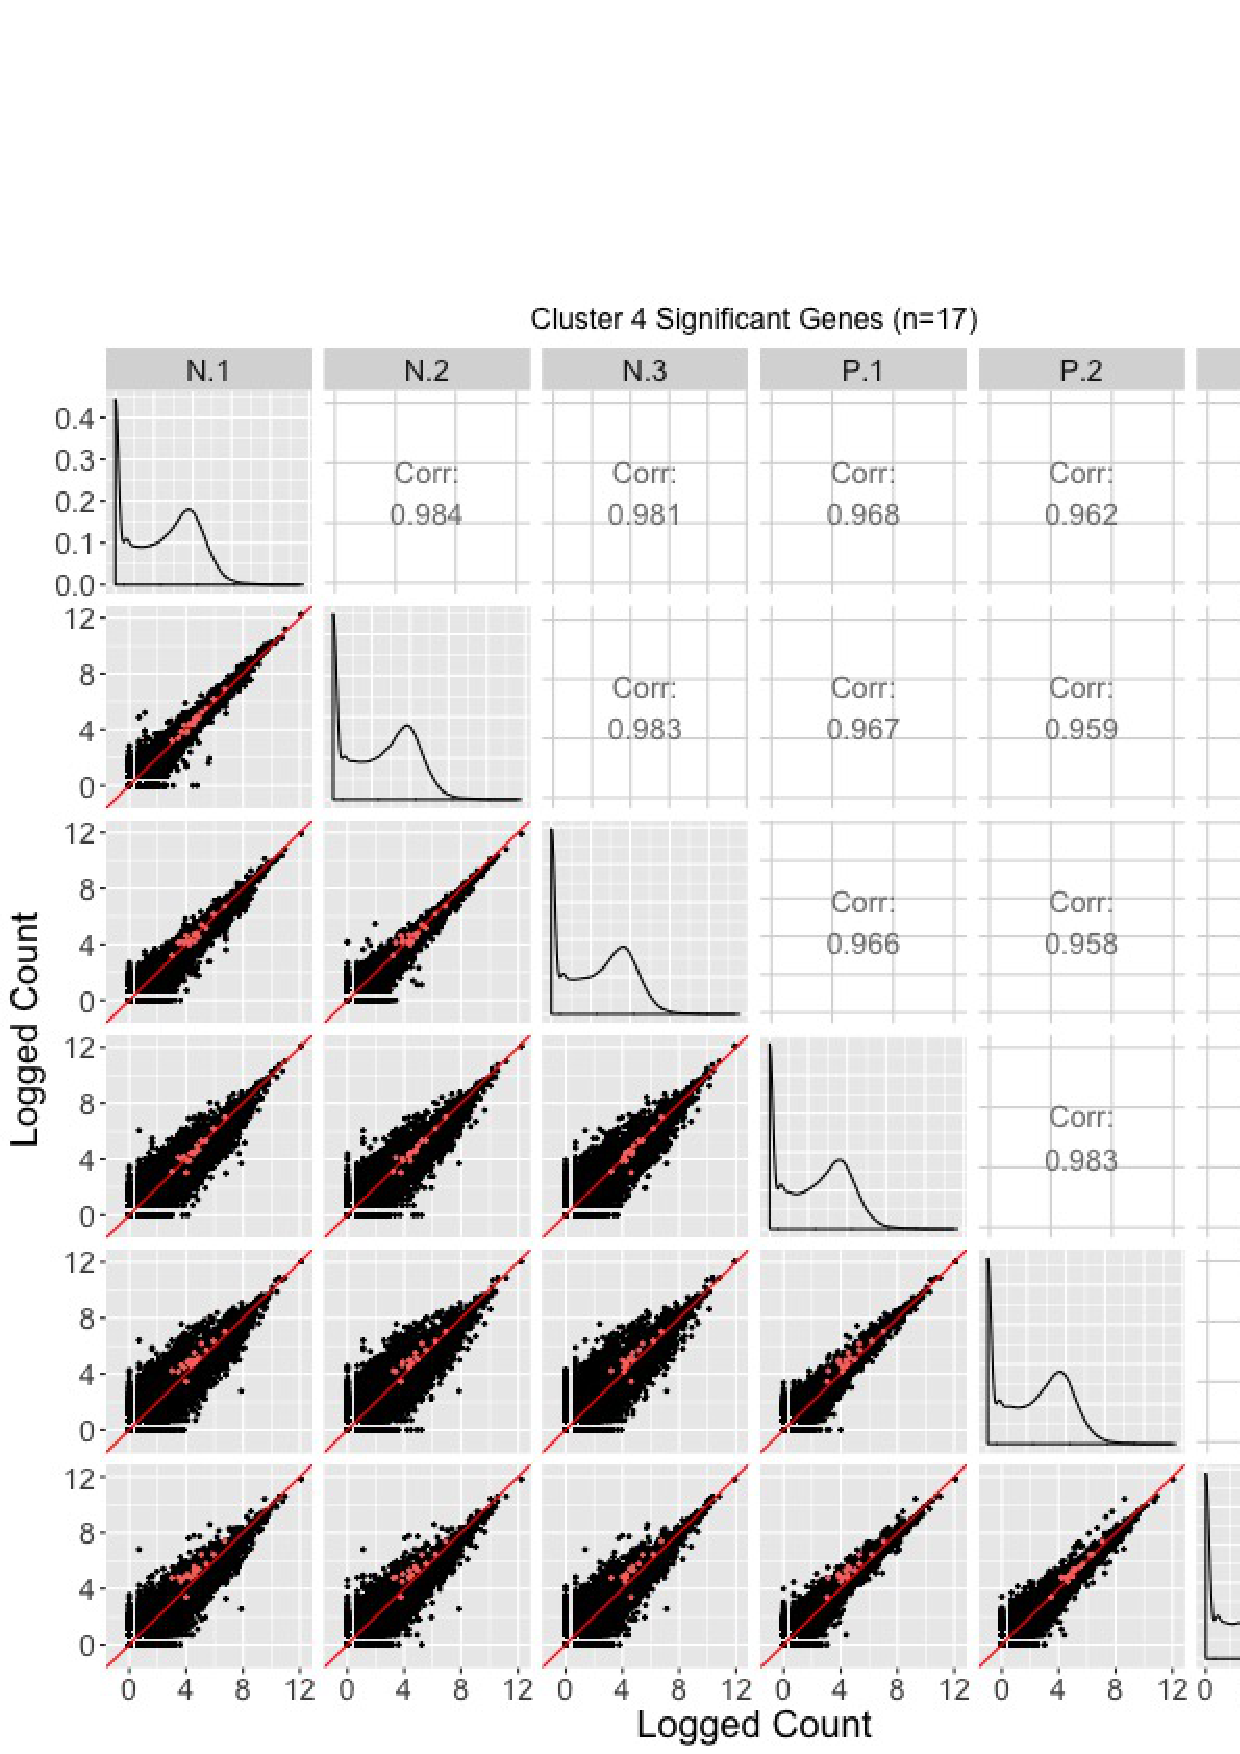
\includegraphics[width=\columnwidth]{../MakeFigures/sbIRClusterSigSM4.jpg}}
  \caption{Example of using a scatterplot matrix to assess DEG calls from a model in the iron-metabolism soybean dataset. There were 17 significant genes in Cluster 4 after performing a hierarchical clustering analysis with a cluster size of four (Figure 2 in the main paper). These significant genes are overlaid in orange on the scatterplot matrix. For the most part, they do not seem to follow the expected patterns of differential expression: In many of the scatterplots between treatments, the orange points do not seem to deviate much from the \textit{x=y} line. Moreover, in the scatterplots between P.1 and P.2 as well as P.1 and P.3, the orange points seems to indicate an underexpression of the P.1 replicate. We similarly saw somewhat messy looking DEG calls in Cluster 4 in the form of parallel coordinate plots (Figure 2 of the main paper) and litre plots (Figure 8 E and F of the main paper).
  \label{sbIRClusterSigSM4}}
  \end{figure}  
  
  \clearpage
  \null 
  \begin{figure}[t!]
  \centerline{\includegraphics[width=0.7\columnwidth]{../MakeFigures/Dashboards/litreCluster1/litreCluster1.jpg}}
  \caption{Litre plots for significant genes inside Cluster 1 from Figure 2 of the paper. Subplots A and B each overlay an example significant gene as nine green points. The genes show patterns expected of differentially-expressed ones, by clumping together and deviating from the \textit{x=y} line. Moreover, the genes appear over-expressed in the P group. This is consistent with what we saw in the parallel coordinate plots of Figure 2 from the main paper. To interactively view the litre plot for all significant genes within Cluster 1, please visit https://rnaseqvisualization.shinyapps.io/litreCluster1.
  \label{litreCluster1}}
  \end{figure}   
  
  
  \clearpage
  The remainder of this supplementary file (Figures~\ref{lkClustersKeep} through~\ref{litreClusterAdd-St}) relates to the application of normalization techniques to the liver and kidney technical replicate data that were introduced in Section 5 (Closing case study) of the main paper. In this case study, technical replicates of kidney and liver RNA-seq data was initially analyzed using library scale normalization. This process lead to 7,050 kidney DEGs and 1,968 liver DEGs, but subsequent visualization analysis suggested that a subset of the kidney DEGs may be unreliable (Figure 10A from the main paper). Upon reviewing the geometrical structure of the data in the form of a scatterplot matrix, a subset of overexpressed liver genes was discovered, implicating the need for a more rigorous form of normalization (Figure 9 from the main paper). As a result, TMM normalization was then applied to the data, which lead to 3,974 kidney DEGs and 3,546 liver DEGs. Ensuing visualization analysis verified that these DEGs now appeared more reliable (Figure 10B from the main paper). \\
  
  In the remaining figures of this supplementary file, we thoroughly explore four subsets of genes from this case study in the form of parallel coordinate plots, scatterplot matrices, and litre plots. We also use variants of some of the techniques introduced in the main paper. Namely, we demonstrate the use of data standardization for scatterplot matrices and litre plots as a means to magnify certain informative patterns at the expense of losing geometrical structure. Throughout the figures below, we use consistent color-coding while plotting example genes from each of the four gene subsets. The four gene subsets and their color-codes are as follows:
  
  \begin{enumerate}
  
  \item The 3,974 kidney-specific DEGs from library scale normalization that remained as DEGs even after TMM normalization. These DEGs are plotted in \textbf{\textcolor{Fuchsia}{\underline{purple}}}. As these genes were declared significant with both library scale normalization and TMM normalization, we expect them to follow the expected patterns of DEGs.
  
  \item The 1,968 liver-specific DEGs from library scale normalization that remained as DEGs even after TMM normalization. These DEGs are plotted in \textbf{\textcolor{Bittersweet}{\underline{orange}}}. As these genes were declared significant with both library scale normalization and TMM normalization, we expect them to follow the expected patterns of DEGs.
  
  \item The 3,076 kidney-specific DEGs from library scale normalization that were \textit{removed} as DEGs using TMM normalization. These DEGs are plotted in \textbf{\textcolor{Red}{\underline{red}}}. As these genes were removed from DEG designation with the more-appropriate TMM normalization, we expect them to \textit{not} convincingly follow the expected patterns of DEGs.
  
  \item The 1,578 liver-specific genes that were not detected as DEGs with library scale normalization but were then \textit{added} as such using TMM normalization. These DEGs are plotted in \textbf{\textcolor{RubineRed}{\underline{pink}}}. As these genes were not declared significant with library scale normalization but were then declared as significant using the more-appropriate TMM normalization, we expect them to \textit{somewhat} convincingly follow the expected patterns of DEGs.
  
  \end{enumerate}
  
  \noindent
  In the remaining twenty figures, the four gene subsets are displayed using each of the following five main plotting approaches:
  
  \begin{enumerate}
  
  \item Figures~\ref{lkClustersKeep} through~\ref{lkClustersAdd} each shows the four gene subsets in the form of parallel coordinate plots after application of hierarchical clustering analysis. Each subset is grouped into eight clusters, not only to separate the genes into any subtle pattern differences, but also to reduce any overplotting that would occur should they all be viewed together as one large cluster. Overall, we see that the genes that were called DEGs in both forms of normalization (purple and orange) have very clean-looking parallel coordinate plots (especially in their largest cluster); the genes that were removed with TMM normalization (red) have messy-looking parallel coordinate plots; and the genes that were added with TMM normalization (pink) have decent-looking parallel coordinate plots.
  
  \item Figures~\ref{lkClustersKeepSM} through~\ref{lkClustersAddSM} each overlays the genes from the largest cluster of the four gene subsets in the form of scatterplot matrices. In general, we see that the genes that were called DEGs in both forms of normalization (purple and orange) have the expected differential expression profiles in the scatterplot matrices, deviating from the \textit{x=y} line in the treatment scatterplots in the anticipated direction. We also see that the genes that were removed with TMM normalization (red) do not show DEG patterns in the scatterplot matrices, as they barely deviate from the \textit{x=y} line in the treatment scatterplots. All three of these gene subsets appear as predicted. However, perhaps surprisingly, the genes that were added with TMM normalization (pink) appear similarly to the genes that were removed with TMM normalization (red). We would expect the pink genes to deviate more from the \textit{x=y} line and demonstrate DEG patterns more than the red genes, but this was not observed. We return to this problem using standardization techniques later in this supplementary file (Figures~\ref{lkClustersRemoveSM-St} and~\ref{lkClustersAddSM-St}).
  
  \item Figures~\ref{litreClusterKeep} through~\ref{litreClusterAdd} each overlays example genes from the largest cluster of the four gene subsets in the form of litre plots. Overall, we see that the example genes that were called DEGs in both forms of normalization (purple and orange) have the expected profiles in the litre plots, deviating as concentrated bundles away from the \textit{x=y} line. We also see that the example genes that were removed with TMM normalization (red) do not show DEG patterns in the litre plots, barely deviating from the \textit{x=y} and/or showing wide dispersion reflecting inconsistent replicates. All three of these gene subsets appear as predicted. However, perhaps surprisingly, the genes that were added with TMM normalization (pink) appear similarly to the genes that were removed with TMM normalization (red). We would expect the pink genes to show DEG patterns (at least more so than the red genes), but this was not observed. We come back to this problem using standardization methods later in this supplementary file (Figures~\ref{litreClusterRemove-St} and~\ref{litreClusterAdd-St}).
  
  \item Figures~\ref{lkClustersKeepSM-St} through~\ref{lkClustersAddSM-St} are the same as Figures~\ref{lkClustersKeepSM} through~\ref{lkClustersAddSM}, only now we \textit{standardized} the data. With standardization, we immediately note that the original geometric structure that elicited meaningful information about the dataset as a whole (variation between treatments and replicates, normalization, sample mislabeling, and unexpected patterns like streaks) is now gone. Instead, the whole dataset appears as an oval-shape that is almost identical across all scatterplots. However, in compensation for losing useful information about the whole dataset, standardization appears to amplify other meaningful patterns in the overlaid DEGs. For instance, just as we saw in Figures~\ref{lkClustersKeepSM} through~\ref{lkClustersAddSM}, the genes that were called DEGs in both forms of normalization (purple and orange) have the expected profiles. However, with standardization, we can see the replicates sticking to the \textit{x=y} line more clearly and we can also see which treatment group is overexpressed more clearly not only in the treatment scatterplots but also in the replicate scatterplots.
  
  \vspace{1mm}
  
  More importantly, while Figures~\ref{lkClustersKeepSM} through~\ref{lkClustersAddSM} showed similar profiles for the genes that were added with TMM normalization (pink) and the genes that were removed with TMM normalization (red), standardization amplifies the differences between the pink and red gene profiles in a manner we would expect. Specifically, the standardized red gene profiles show widely dispersed genes that sometimes deviate from the \textit{x=y} line in the replicate scatterplots and cross both sides of and sometimes stick to the \textit{x=y} line in the treatment scatterplots (Figure~\ref{lkClustersRemoveSM-St}). In other words, the red gene profiles often show patterns not akin to differential expression, which we would expect from genes that were \textit{removed} as DEGs with TMM normalization. In contrast, the standardized pink gene profiles show less-widely dispersed genes that deviate less from the \textit{x=y} line in the replicate scatterplots and deviate more from the \textit{x=y} line in the treatment scatterplots (Figure~\ref{lkClustersAddSM-St}). In other words, the pink gene profiles show patterns more akin to differential expression than the red genes, which we would expect from genes that were \textit{added} as DEGs with TMM normalization. At the same time, the pink gene profiles are not as clean-looking as the purple and orange genes that were designated as DEGs in both forms of normalization. Overall, in these standardized scatterplot matrices, the pink genes appear as an intermediate between the clean-looking purple and orange genes and the messy-looking red genes, which we might expect.
  
  \item Figures~\ref{litreClusterKeep-St} through~\ref{litreClusterAdd-St} are the same as Figures~\ref{litreClusterKeep} through~\ref{litreClusterAdd}, only now we \textit{standardized} the data. With standardization, we immediately note that the original geometric structure in the hexagonal binning that elicited meaningful information about the problematic streak of over-expressed liver genes is now gone. Instead, the dataset appears as an oval-shape in the hexagonal binning. Just as we saw in Figures~\ref{litreClusterKeep} through~\ref{litreClusterAdd}, the genes that were called DEGs in both forms of normalization (purple and orange) have the expected profiles.
  
  \clearpage
  
  Notably, while Figures~\ref{litreClusterKeep} through~\ref{litreClusterAdd} showed similar profiles for the example genes that were removed with TMM normalization (red) and the example genes that were added with TMM normalization (pink), standardization amplifies the differences between the red and pink gene profiles in a manner we would expect. For example, we provide standardized litre plots for the nine genes with the lowest FDR values for both the red (Figure~\ref{litreClusterRemove-St}) and pink (Figure~\ref{litreClusterAdd-St}) groups, and we can quickly determine that the pink profiles show patterns more akin to differential expression than the red groups. Namely, the overlaid pink points deviate more from the \textit{x=y} line in a tight cluster than the overlaid red points. At the same time, the overlaid pink points show patterns less akin to differential expression than the purple and orange points. All together, the pink gene profiles appear as an intermediate between the clean-looking purple and orange genes and the messy-looking red genes in the standardized litre plots, which is to be expected if TMM normalization is the more appropriate technique.
  
  \end{enumerate}
  
  \null
  \begin{figure}[t!]
  \centerline{\includegraphics[width=0.65\columnwidth]{../MakeFigures/lkClustersKeep.jpg}}
  \caption{Parallel coordinate plots showing eight hierarchical clusters from the 3,974 genes that remained in the kidney-specific DEGs after TMM normalization. We see that, for the most part, the parallel coordinate patterns follow the expected patterns across the clusters. The ideal pattern of DEGs is especially captured in the first cluster (the largest one with 1,136 genes). We applied ombre coloring across the clusters in order of cluster size. We used hierarchical clustering to tease apart subtle pattern differences and to mitigate additional overplotting that would occur if we were to plot all genes onto only one parallel coordinate plot. The side-by-side boxplots represent \textit{all} gene counts in the dataset.
  \label{lkClustersKeep}}
  \end{figure}
  
  \null
  \begin{figure}[t!]
  \centerline{\includegraphics[width=0.65\columnwidth]{../MakeFigures/lkClustersOrig.jpg}}
  \caption{Parallel coordinate plots showing eight hierarchical clusters from the 1,968 genes that remained in the liver-specific DEGs after TMM normalization. We see that, for the most part, the parallel coordinate patterns follow the expected patterns across the clusters. The ideal pattern of DEGs is especially captured in the first cluster (the largest one with 933 genes). We applied ombre coloring across the clusters in order of cluster size. We used hierarchical clustering to tease apart subtle pattern differences and to mitigate additional overplotting that would occur if we were to plot all genes onto only one parallel coordinate plot. The side-by-side boxplots represent \textit{all} gene counts in the dataset.
  \label{lkClustersOrig}}
  \end{figure}
  
  \null
  \begin{figure}[t!]
  \centerline{\includegraphics[width=0.65\columnwidth]{../MakeFigures/lkClustersRemove.jpg}}
  \caption{Parallel coordinate plots showing eight hierarchical clusters from the 3,076 genes that were removed from the kidney-specific DEGs after TMM normalization. The patterns in almost all clusters do not resemble the expected DEG format; instead, they show large variability between replicates and small variability between treatments. In some clusters, it is difficult to even determine which group would be the overexpressed one if its genes were in fact DEGs. Taken together, this plot provides additional statistical evidence that the application of TMM normalization successfully removed genes that were previously mislabeled as kidney-specific DEGs with library scaling normalization. We applied ombre coloring across the clusters in order of cluster size. We used hierarchical clustering to tease apart subtle pattern differences and to mitigate overplotting. The side-by-side boxplots represent \textit{all} gene counts in the dataset.
  \label{lkClustersRemove}}
  \end{figure}
  
  \null
  \begin{figure}[t!]
  \centerline{\includegraphics[width=0.65\columnwidth]{../MakeFigures/lkClustersAdd.jpg}}
  \caption{Parallel coordinate plots showing eight hierarchical clusters from the 1,578 genes that were \textit{added} as liver-specific DEGs after TMM normalization. We see that, for the most part, the parallel coordinate lines follow the expected patterns across the clusters, but not as precisely as we saw with the purple (Figure~\ref{lkClustersKeep}) and orange (Figure~\ref{lkClustersOrig}) gene subsets. We applied ombre coloring across the clusters in order of cluster size. We used hierarchical clustering to tease apart subtle pattern differences and to mitigate additional overplotting that would occur if we were to plot all genes onto only one parallel coordinate plot. The side-by-side boxplots represent \textit{all} gene counts in the dataset.
  \label{lkClustersAdd}}
  \end{figure}
  
  \null
  \begin{figure}[t!]
  \centerline{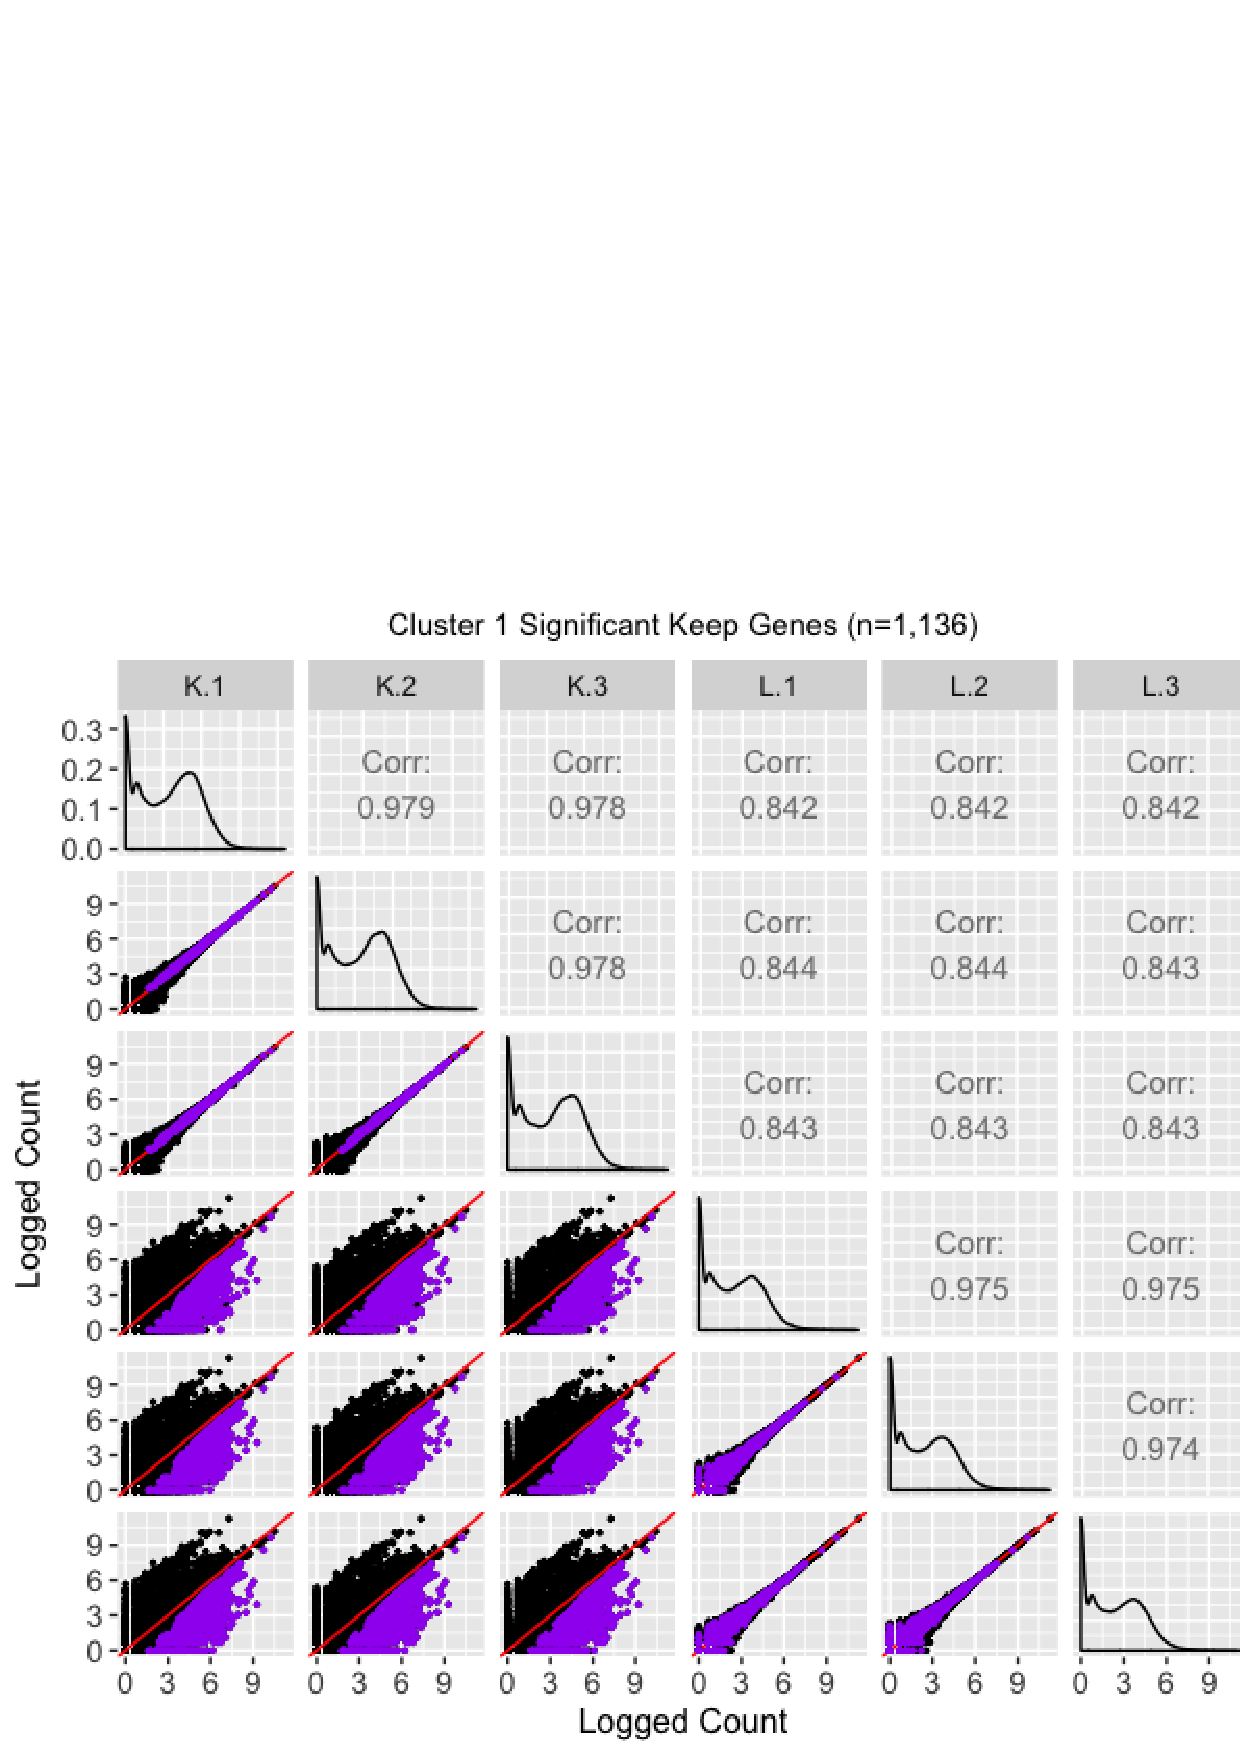
\includegraphics[width=1\columnwidth]{../MakeFigures/lkClustersKeepSM.jpg}}
  \caption{Scatterplot matrix of the 1,136 genes that were in the first cluster (of Figure~\ref{lkClustersKeep}) from genes that remained as kidney-specific DEGs even after TMM normalization. With this scatterplot matrix, we verify from an additional perspective that these genes demonstrate the expected patterns of DEGs.
  \label{lkClustersKeepSM}}
  \end{figure}
  
  \null
  \begin{figure}[t!]
  \centerline{\includegraphics[width=1\columnwidth]{../MakeFigures/lkClustersOrigSM.jpg}}
  \caption{Scatterplot matrix of the 933 genes that were in the first cluster (of Figure~\ref{lkClustersOrig}) from genes that remained as liver-specific DEGs even after TMM normalization. With this scatterplot matrix, we verify from an additional perspective that these genes demonstrate the expected patterns of DEGs.
  \label{lkClustersOrigSM}}
  \end{figure}
  
  \null
  \begin{figure}[t!]
  \centerline{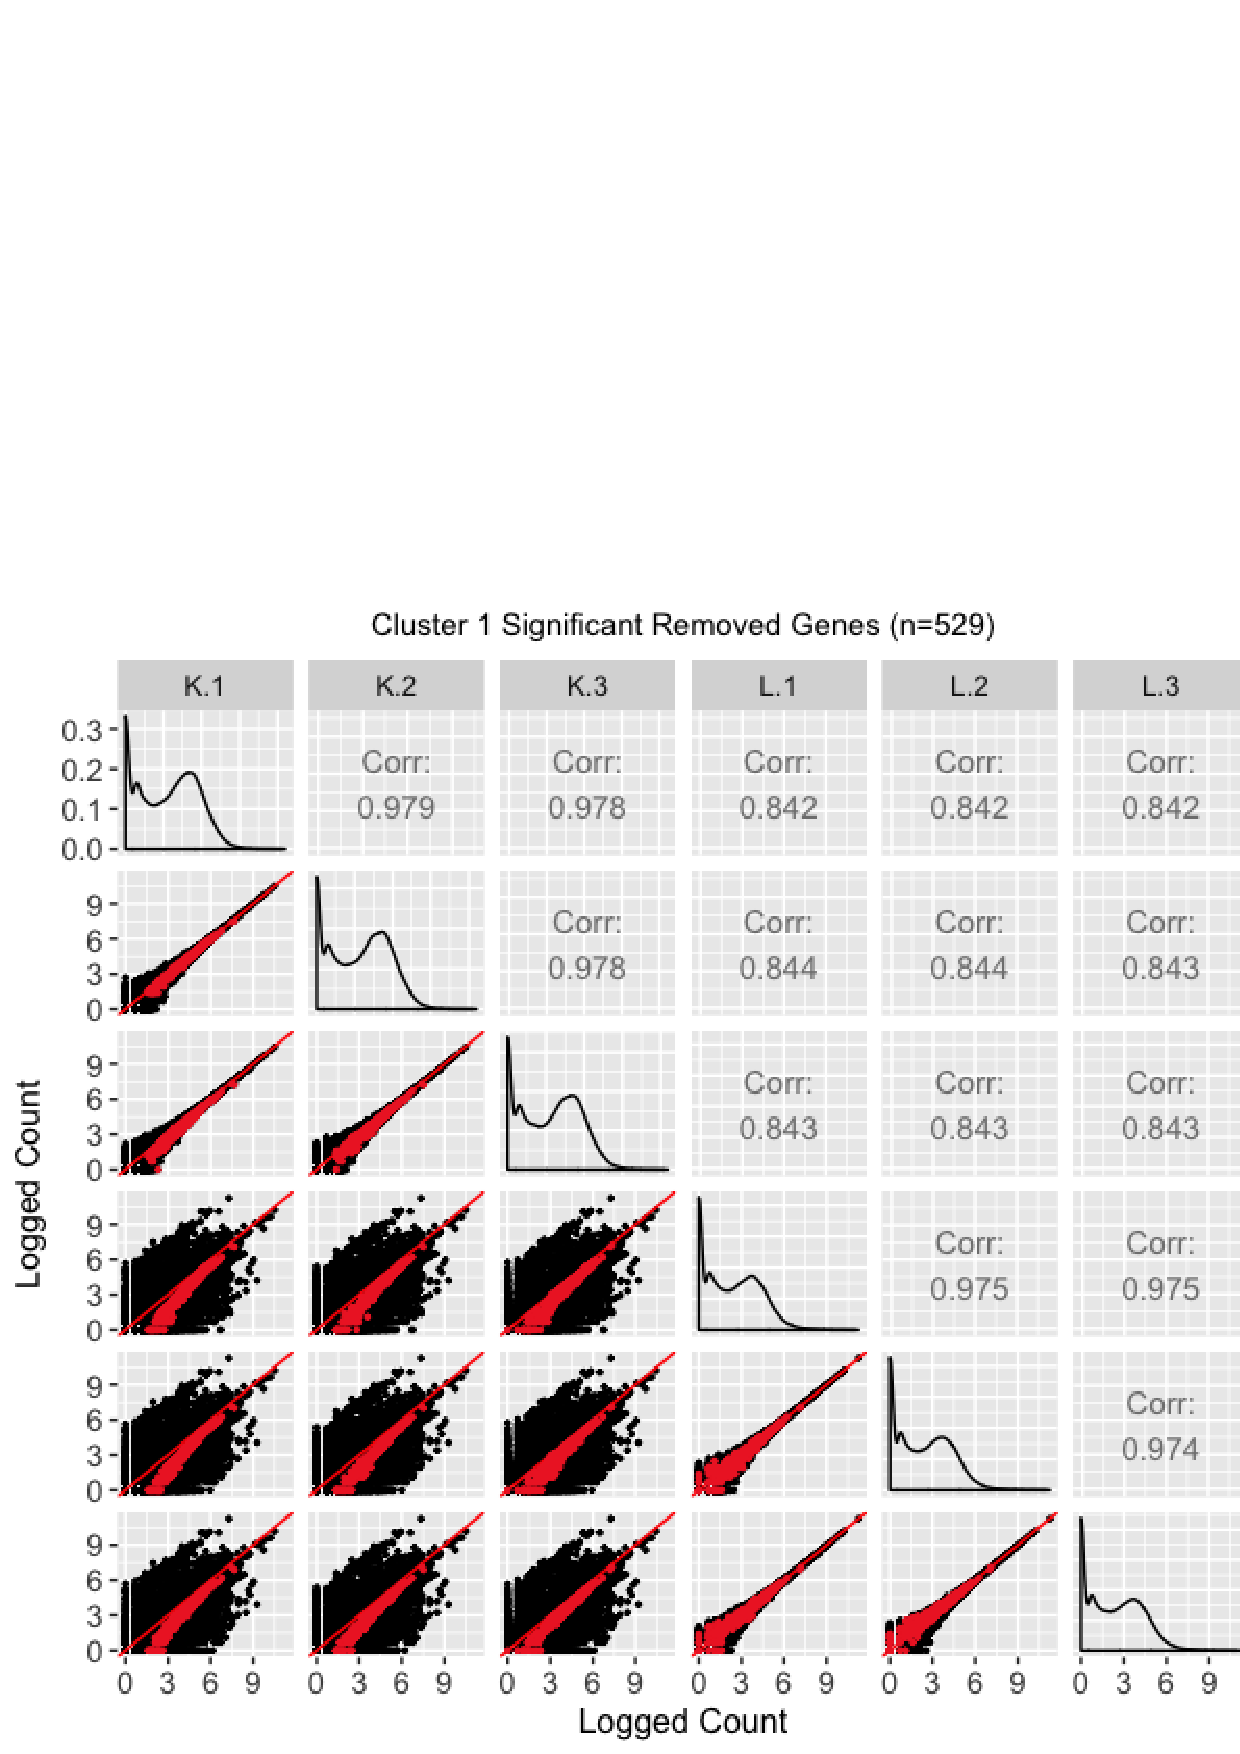
\includegraphics[width=1\columnwidth]{../MakeFigures/lkClustersRemoveSM.jpg}}
  \caption{Scatterplot matrix of the 529 genes that were in the first cluster (of Figure~\ref{lkClustersRemove}) from genes that no longer remained as kidney-specific DEGs after TMM normalization. With this scatterplot matrix, we verify from an additional perspective that these genes do \textit{not} demonstrate the expected patterns of DEGs too strongly (they do not deviate much from the \textit{x=y} line in the treatment scatterplots). This provides additional evidence that TMM normalization removing these genes from DEG status may be valid.
  \label{lkClustersRemoveSM}}
  \end{figure}
  
  \null
  \begin{figure}[t!]
  \centerline{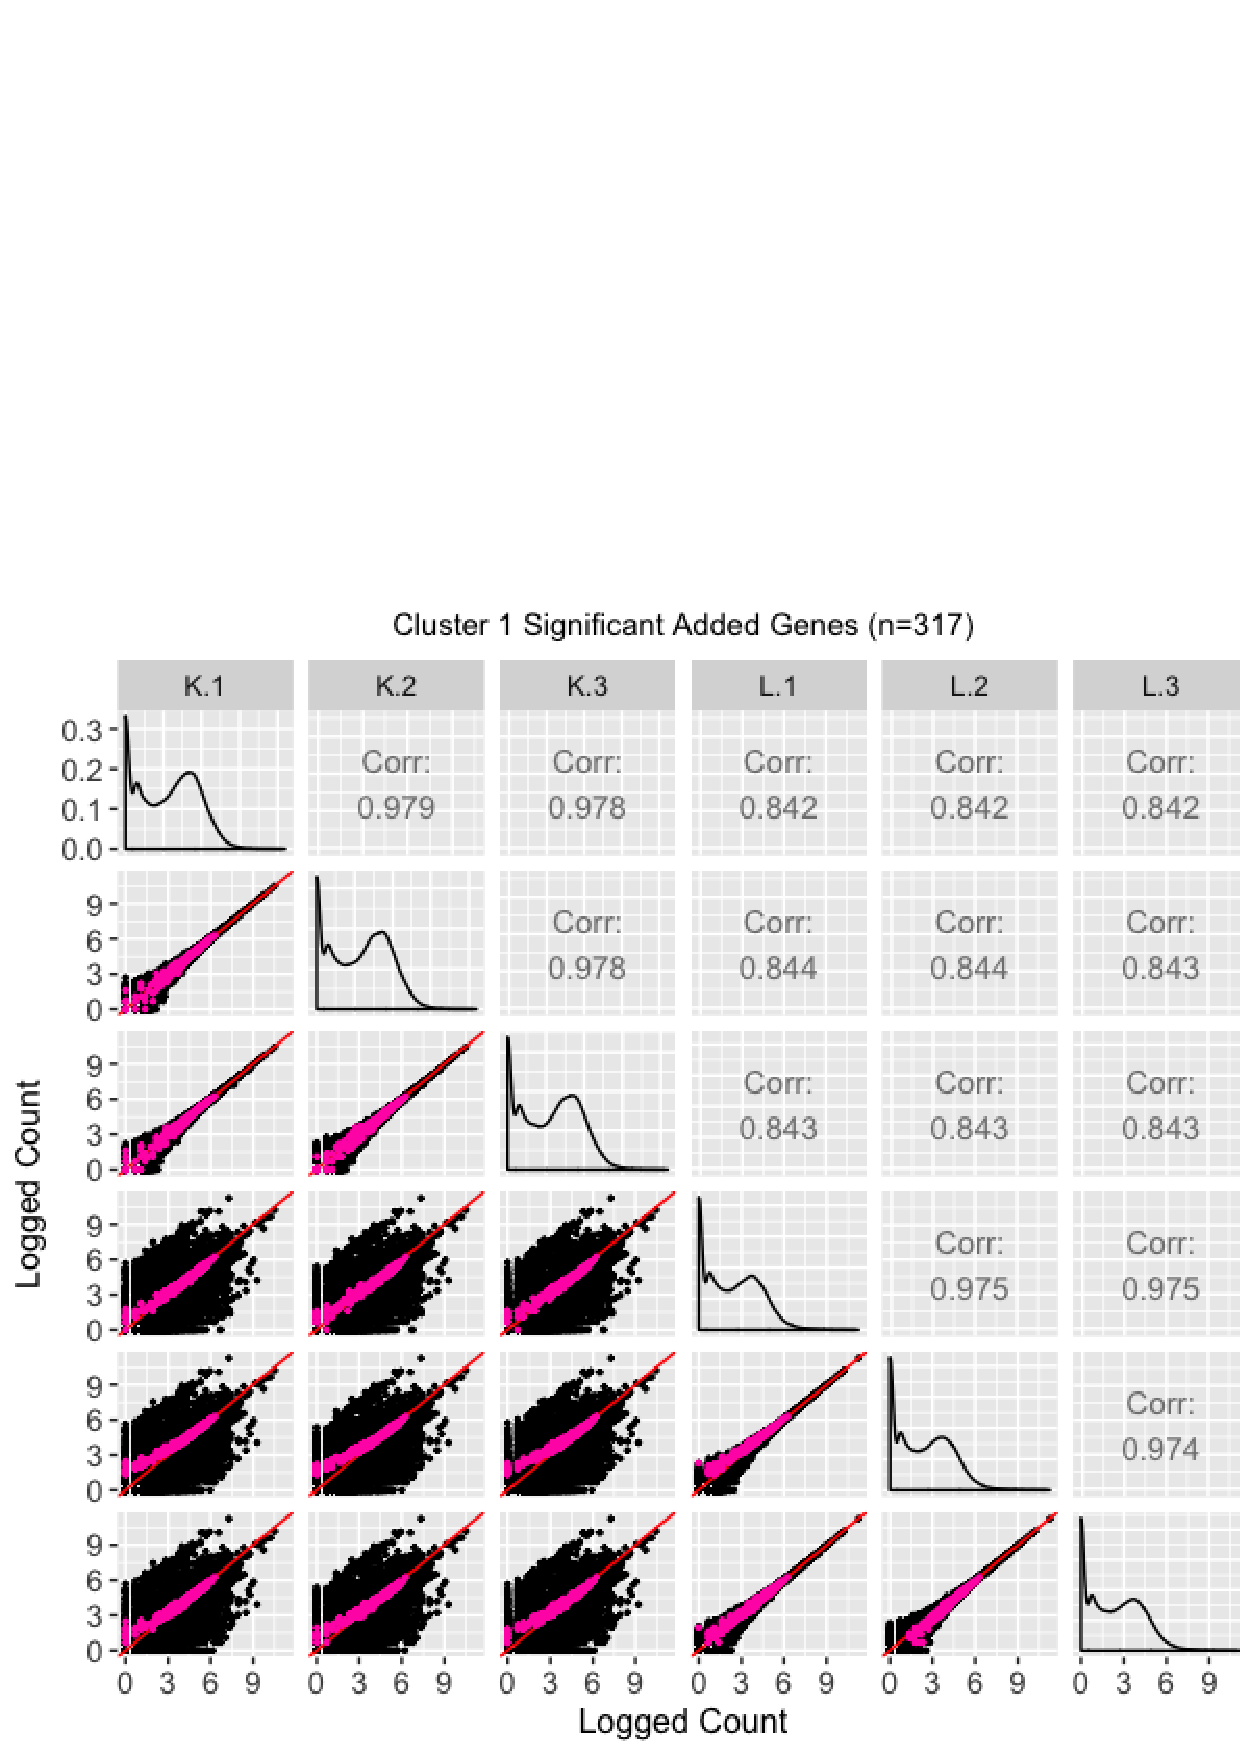
\includegraphics[width=1\columnwidth]{../MakeFigures/lkClustersAddSM.jpg}}
  \caption{Scatterplot matrix of the 317 genes that were in the first cluster (of Figure~\ref{lkClustersAdd}) from genes that were \textit{added} as liver-specific DEGs after TMM normalization. With this scatterplot matrix, we see that the genes do \textit{not} demonstrate the expected patterns of DEGs too strongly (they do not deviate much from the \textit{x=y} line in the treatment scatterplots). In fact, these pink genes appear similarly to what we saw from the scatterplot matrix of the red genes (Figure~\ref{lkClustersRemoveSM}). This is somewhat of a surprise, given that the pink genes were \textit{added} by TMM  normalization, while the red genes were \textit{removed} by TMM normalization. Stated differently, we would expect the pink genes to appear more like differentially expressed genes if TMM normalization is appropriate, but we could not confirm this expectation. We will return to this problem using standardization techniques later in the supplementary file (Figures~\ref{lkClustersRemoveSM-St} and~\ref{lkClustersAddSM-St}).
  \label{lkClustersAddSM}}
  \end{figure}
  
  
  \null
  \begin{figure}[t!]
  \centerline{\includegraphics[width=0.7\columnwidth]{../MakeFigures/Dashboards/litreClusterKeep/litreClusterKeep.jpg}}
  \caption{Example litre plots from the 1,136 genes that were in the first cluster (Figure~\ref{lkClustersKeep}) of genes that remained as kidney-specific DEGs even after TMM normalization. With these litre plots, we verify from an additional perspective that these genes demonstrate the expected patterns of DEGs.
  \label{litreClusterKeep}}
  \end{figure}
  
  \null
  \begin{figure}[t!]
  \centerline{\includegraphics[width=0.7\columnwidth]{../MakeFigures/Dashboards/litreClusterOrig/litreClusterOrig.jpg}}
  \caption{Example litre plots from the 933 genes that were in the first cluster (Figure~\ref{lkClustersOrig}) from genes that remained as liver-specific DEGs even after TMM normalization. With these litre plots, we verify from an additional perspective that these genes demonstrate the expected patterns of DEGs.
  \label{litreClusterOrig}}
  \end{figure}
  
  \null
  \begin{figure}[t!]
  \centerline{\includegraphics[width=0.7\columnwidth]{../MakeFigures/Dashboards/litreClusterRemove/litreClusterRemove.jpg}}
  \caption{Example litre plots from the 529 genes that were in the first cluster (Figure~\ref{lkClustersRemove}) of genes that no longer remained as kidney-specific DEGs after TMM normalization. With these litre plots, we verify from an additional perspective that these genes do not demonstrate the expected patterns of DEGs. This provides additional evidence that TMM normalization removing these genes from DEG status may be valid.
  \label{litreClusterRemove}}
  \end{figure}
  
  \null
  \begin{figure}[t!]
  \centerline{\includegraphics[width=0.7\columnwidth]{../MakeFigures/Dashboards/litreClusterAdd/litreClusterAdd.jpg}}
  \caption{Example litre plots from the 317 genes that were in the first cluster (Figure~\ref{lkClustersAdd}) from genes that were \textit{added} as liver-specific DEGs after TMM normalization. With these litre plots, we see that the genes do \textit{not} demonstrate the expected patterns of DEGs in a trustworthy manner. In fact, these pink genes appear similarly to what we saw from the example litre plots of the red genes (Figure~\ref{litreClusterRemove}). This is somewhat of a surprise, given that the pink genes were \textit{added} by TMM  normalization, while the red genes were \textit{removed} by TMM normalization. Stated differently, we would expect the pink genes to appear more like differentially expressed genes if TMM normalization is appropriate, but we could not confirm this expectation. We will return to this problem using standardization techniques later in the supplementary file (Figures~\ref{litreClusterRemove-St} and~\ref{litreClusterAdd-St}).
  \label{litreClusterAdd}}
  \end{figure}
  
  \null
  \begin{figure}[t!]
  \centerline{\includegraphics[width=1\columnwidth]{../MakeFigures/lkClustersKeepSM-St.jpg}}
  \caption{Scatterplot matrix of the \textit{standardized} 1,136 genes that were in the first cluster (Figure~\ref{lkClustersKeep}) from genes that remained as kidney-specific DEGs even after TMM normalization. Even though the standardization process removes the interesting geometrical features we saw back in Figure~\ref{lkClustersKeepSM} regarding the streak of overexpressed liver genes, it amplifies other patterns in meaningful ways. For instance, compared to Figure~\ref{lkClustersKeepSM}, the highlighted genes here appear more clustered and separated from the \textit{x=y} line in the treatment scatterplots, and more clustered and connected to the \textit{x=y} line in the replicate scatterplots. We can also now see more clearly in the replicate scatterplots that the kidney expression is higher than the liver expression.
  \label{lkClustersKeepSM-St}}
  \end{figure}
  
  \null
  \begin{figure}[t!]
  \centerline{\includegraphics[width=1\columnwidth]{../MakeFigures/lkClustersOrigSM-St.jpg}}
  \caption{Scatterplot matrix of the \textit{standardized} 933 genes that were in the first cluster (Figure~\ref{lkClustersOrig}) from genes that remained as liver-specific DEGs even after TMM normalization. Even though the standardization process removes the interesting geometrical features we saw back in Figure~\ref{lkClustersOrigSM} regarding the streak of overexpressed liver genes, it amplifies other patterns in meaningful ways. For instance, compared to Figure~\ref{lkClustersOrigSM}, the highlighted genes here appear more clustered and separated from the \textit{x=y} line in the treatment scatterplots, and more clustered and connected to the \textit{x=y} line in the replicate scatterplots. We can also now see more clearly in the replicate scatterplots that the liver expression is higher than the kidney expression. 
  \label{lkClustersOrigSM-St}}
  \end{figure}
  
  \null
  \begin{figure}[t!]
  \centerline{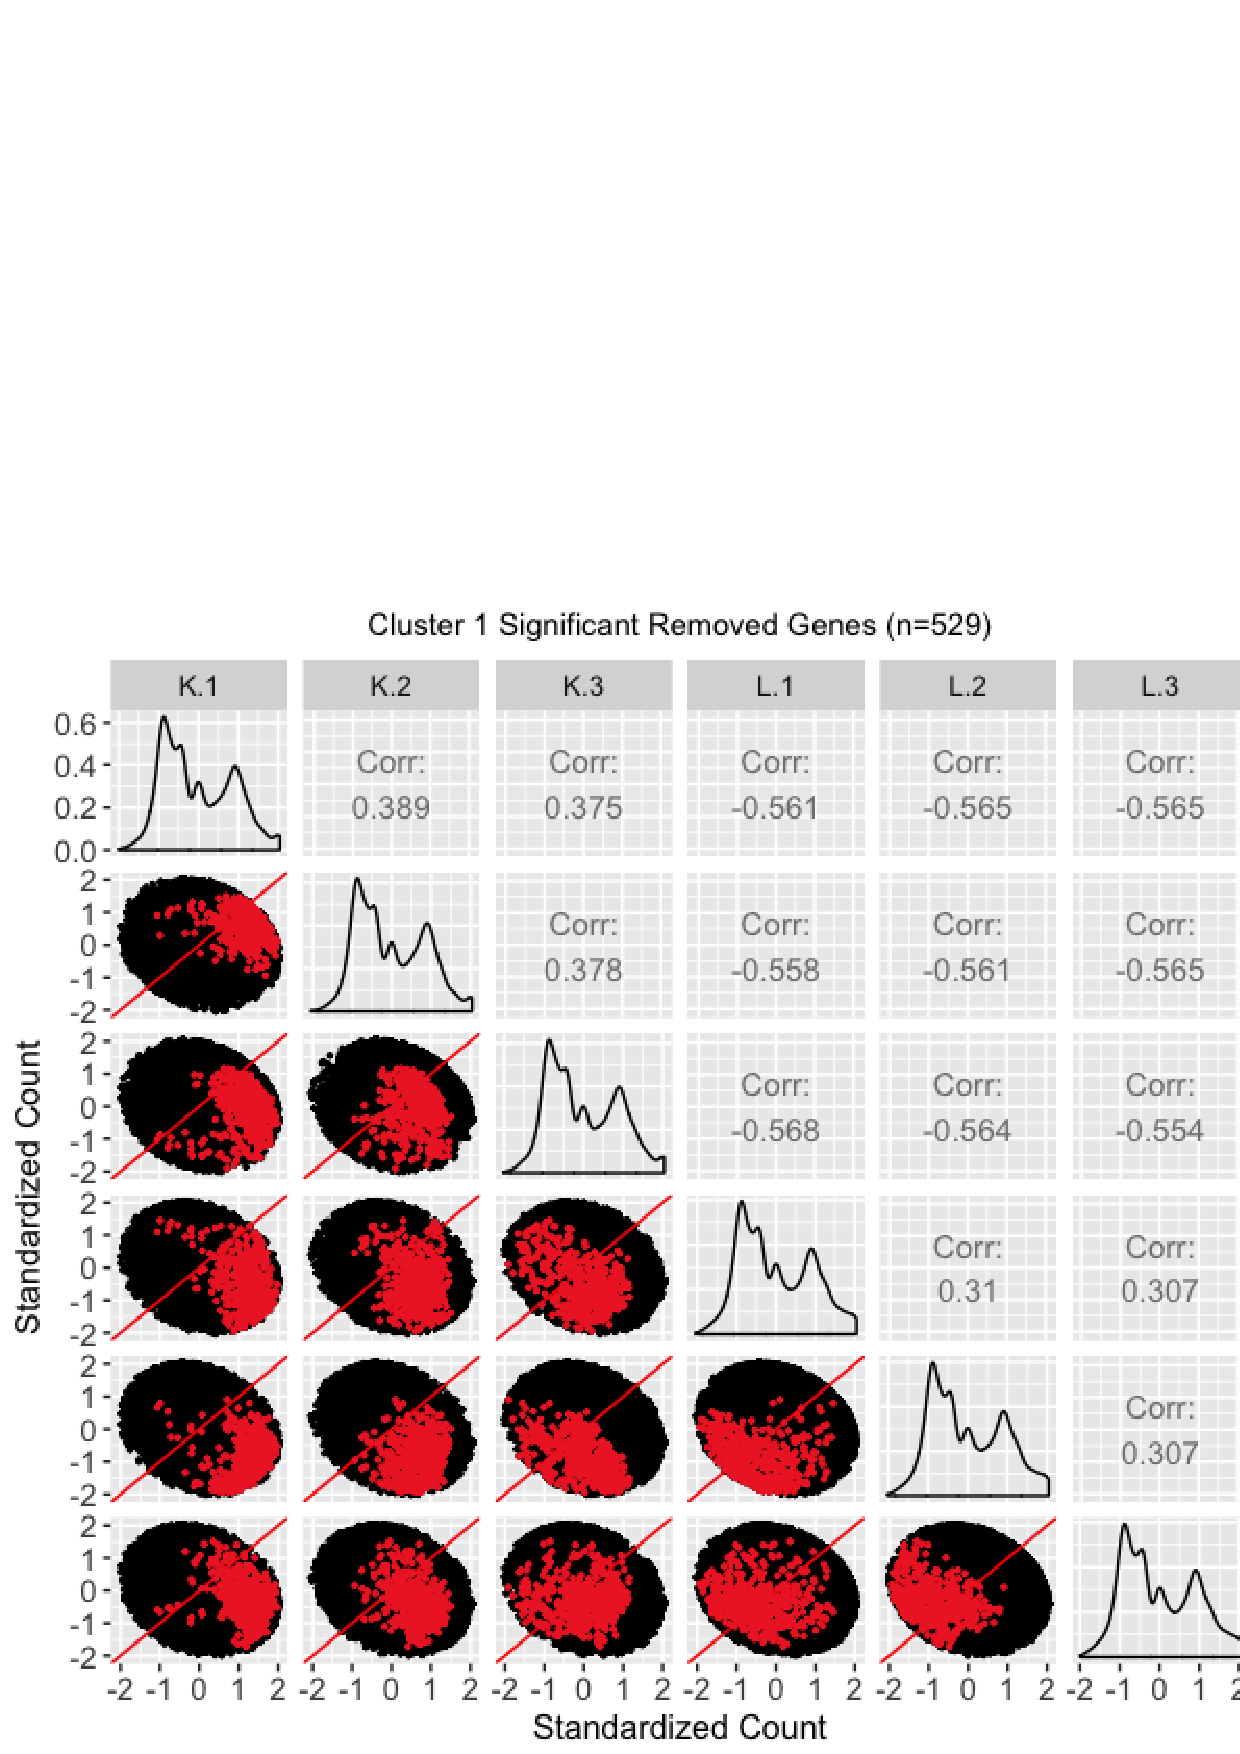
\includegraphics[width=1\columnwidth]{../MakeFigures/lkClustersRemoveSM-St.jpg}}
  \caption{Scatterplot matrix of the \textit{standardized} 529 genes that were in the first cluster (Figure~\ref{lkClustersRemove}) from genes that no longer remained as kidney-specific DEGs after TMM normalization. Even though the standardization process removes the interesting geometrical features we saw back in Figure~\ref{lkClustersRemoveSM} regarding the streak of overexpressed liver genes, it allows us to view the DEG patterns in a different meaningful fashion. Namely, the genes of interest are now spread out more, and the replicate and treatment scatterplots are almost indistinguishable from each other, with both of them showing genes of interest crossing both sides of the \textit{x=y} line. In other words, standardization of the data provides additional visualization evidence that TMM normalization was justified in removing these genes from DEG designation. 
  \label{lkClustersRemoveSM-St}}
  \end{figure}
  
  \null
  \begin{figure}[t!]
  \centerline{\includegraphics[width=1\columnwidth]{../MakeFigures/lkClustersAddSM-St.jpg}}
  \caption{Scatterplot matrix of the \textit{standardized} 317 genes that were in the first cluster (Figure~\ref{lkClustersAdd}) from genes that were \textit{added} as liver-specific DEGs after TMM normalization. Even though the standardization process removes the interesting geometrical features we saw back in Figure~\ref{lkClustersAddSM} regarding the streak of overexpressed liver genes, it allows us to view the DEG patterns in a different meaningful fashion. Namely, the genes of interest are now spread out more, and we can now distinguish the replicate and treatment scatterplots more clearly. For the most part, the genes of interest deviate from the \textit{x=y} line in the treatment scatterplots more so than in the replicate scatterplots, and hence display somewhat of the pattern of differential expression. In fact, the pink genes again appear as an intermediate between the purple and orange genes that clearly display differential expression (Figures~\ref{lkClustersKeepSM-St} and~\ref{lkClustersOrigSM-St}) and the red genes that clearly do \textit{not} display differential expression (Figure~\ref{lkClustersRemoveSM-St}). In other words, standardized scatterplot matrices provide additional visualization evidence that TMM normalization was justified in removing the red genes from and adding the pink genes to DEG designation.
  \label{lkClustersAddSM-St}}
  \end{figure}
  
  \null
  \begin{figure}[t!]
  \centerline{\includegraphics[width=0.7\columnwidth]{../MakeFigures/Dashboards/litreClusterKeep-St/litreClusterKeep-St.jpg}}
  \caption{Example \textit{standardized} litre plots from the 1,136 genes that were in the first cluster (Figure~\ref{lkClustersKeep}) of genes that remained as kidney-specific DEGs even after TMM normalization. With standardization, we immediately note that meaningful information about the dataset as a whole (variation between treatments and replicates, normalization, sample mislabeling, and unexpected patterns like streaks) is now gone. However, we confirm that these standardized litre plots corroborate the corresponding non-standardized litre plots we saw in Figure~\ref{litreClusterKeep} that these purple genes demonstrate the expected patterns of DEGs.
  \label{litreClusterKeep-St}}
  \end{figure}
  
  \null
  \begin{figure}[t!]
  \centerline{\includegraphics[width=0.7\columnwidth]{../MakeFigures/Dashboards/litreClusterOrig-St/litreClusterOrig-St.jpg}}
  \caption{Example litre plots from the 933 genes that were in the first cluster (Figure~\ref{lkClustersOrig}) from genes that remained as liver-specific DEGs even after TMM normalization. With standardization, we immediately note that meaningful information about the dataset as a whole (variation between treatments and replicates, normalization, sample mislabeling, and unexpected patterns like streaks) is now gone. However, we confirm that these standardized litre plots corroborate the corresponding non-standardized litre plots we saw in Figure~\ref{litreClusterOrig} that these orange genes demonstrate the expected patterns of DEGs.
  \label{litreClusterOrig-St}}
  \end{figure}
  
  \null
  \begin{figure}[t!]
  \centerline{\includegraphics[width=\columnwidth]{../MakeFigures/Dashboards/litreClusterRemove-St/litreClusterRemove-St.jpg}}
  \caption{\textit{Standardized} litre plots for the nine genes with the lowest FDR values out of the 529 genes that were in the first cluster (Figure~\ref{lkClustersRemove}) of genes that no longer remained as kidney-specific DEGs after TMM normalization. As with the corresponding non-standardized litre plots in Figure~\ref{litreClusterRemove}, we verify from an additional perspective that the red genes do not demonstrate the expected patterns of DEGs. The example red genes here are show much larger inconsistencies between replicates than what we saw with the purple (Figure~\ref{litreClusterKeep-St}) and orange (Figure~\ref{litreClusterOrig-St}) genes. This provides additional evidence that TMM normalization removing these genes from DEG status may be valid.
  \label{litreClusterRemove-St}}
  \end{figure}
  
  \null
  \begin{figure}[t!]
  \centerline{\includegraphics[width=\columnwidth]{../MakeFigures/Dashboards/litreClusterAdd-St/litreClusterAdd-St.jpg}}
  \caption{\textit{Standardized} litre plots for the nine genes with the lowest FDR values out of the 317 genes that were in the first cluster (Figure~\ref{lkClustersAdd}) from genes that were \textit{added} as liver-specific DEGs after TMM normalization. While non-standardized litre plots showed similar profiles between the red (Figure~\ref{litreClusterRemove}) and pink (Figure~\ref{litreClusterAdd}) genes, standardization amplifies the differences in a manner we would expect. Namely, we can now quickly determine that the pink profiles in this figure show patterns more akin to differential expression than the red profiles in Figure~\ref{litreClusterRemove-St}. That is, the overlaid pink points deviate more from the \textit{x=y} line in a tight cluster than the overlaid red points. At the same time, the overlaid pink points here show patterns less akin to differential expression than the purple (Figure~\ref{litreClusterKeep-St}) and orange (Figure~\ref{litreClusterOrig-St}) points. All together, the standardized litre plots place the pink gene profiles as an intermediate between the clean-looking purple and orange genes and the messy-looking red genes, which is to be expected if TMM normalization is the more appropriate technique.
  \label{litreClusterAdd-St}}
  \end{figure}
  
  \end{document}